\documentclass[10pt,twocolumn,letterpaper]{article}

\usepackage{cvpr}
\usepackage{times}
\usepackage{epsfig}
\usepackage{graphicx}
\usepackage{amsmath}
\usepackage{amssymb}

% Include other packages here, before hyperref.

% If you comment hyperref and then uncomment it, you should delete
% egpaper.aux before re-running latex.  (Or just hit 'q' on the first latex
% run, let it finish, and you should be clear).
\usepackage[breaklinks=true,bookmarks=false]{hyperref}

\cvprfinalcopy % *** Uncomment this line for the final submission

\def\cvprPaperID{****} % *** Enter the CVPR Paper ID here
\def\httilde{\mbox{\tt\raisebox{-.5ex}{\symbol{126}}}}

% Pages are numbered in submission mode, and unnumbered in camera-ready
%\ifcvprfinal\pagestyle{empty}\fi
\setcounter{page}{1}
\begin{document}

%%%%%%%%% TITLE
\title{Self-Driving Car Steering Angle Prediction Based on Image Recognition (Milestone)}

\author{Shuyang Du\\
{\tt\small shuyangd@stanford.edu}
% For a paper whose authors are all at the same institution,
% omit the following lines up until the closing ``}''.
% Additional authors and addresses can be added with ``\and'',
% just like the second author.
% To save space, use either the email address or home page, not both
\and
Haoli Guo\\
{\tt\small haoliguo@stanford.edu}
\and
Andrew Simpson\\
{\tt\small asimpso8@stanford.edu}
}

\maketitle
%\thispagestyle{empty}

%%%%%%%%% ABSTRACT
\begin{abstract}
Self-driving vehicles have expanded dramatically over the last few years. Udacity has release a dataset containing, among other data, a set of images with the steering angle captured during driving. The Udacity challenge aimed to predict steering angle based on only the provided images. 

We explore different models to perform high quality prediction of steering angles based on images using different deep learning techniques including Transfer Learning, 3D CNN, LSTM and ResNet. In addition to predicting steering angle, we also predict auxiliary variables like torque and speed to make the model know better about the driving condition and thus produce precise steering angle predictions.

\end{abstract}

%%%%%%%%% BODY TEXT
\section{Introduction}
Self-driving vehicles are going to be of enormous economic impact over the coming decade. Creating models that meet or exceed the ability of a human driver could save thousands of lives a year. Udacity has an ongoing challenge to create an open source self-driving car. In their second challenge Udacity released a dataset of images taken while driving along with the corresponding steering angle and ancillary sensor data for a training set (left, right, and center cameras with interpolated angles based on camera angle). The goal of the challenge was to find a model that, given an image taken while driving, will minimize the RMSE (root mean square error) between what the model predicts and the actual steering angle produced by a human driver. In this project, we explore a variety of techniques including 3D convolutional neural networks, recurrent neural networks using LSTM, ResNets, etc. to output a predicted steering angle in numerical values.

The motivation of the project is to eliminate the need for hand-coding rules and instead create a system that learns how to drive by observing. Predicting steering angle is one important part of the end-to-end approach to self-driving car and would allow us to explore the full power of neural networks. For example, using only steering angle as the training signal, deep neural networks can automatically extract features to help position the road to make the prediction.


%-------------------------------------------------------------------------
\section{Related Work}

NVIDIA released a paper last year "End to End Learning for Self-Driving Cars" \cite{bojarski2016end}. In this paper the authors used a relatively basic CNN architecture. The layout of the architecture can be seen in Figure \ref{nvidiaimage}. Augmentation of the data collected was found to be important. The authors used artificial shifts and rotations of the training set. Left and right cameras with interpolated steering angles were also incorporated.
\begin{figure}[!htb]
	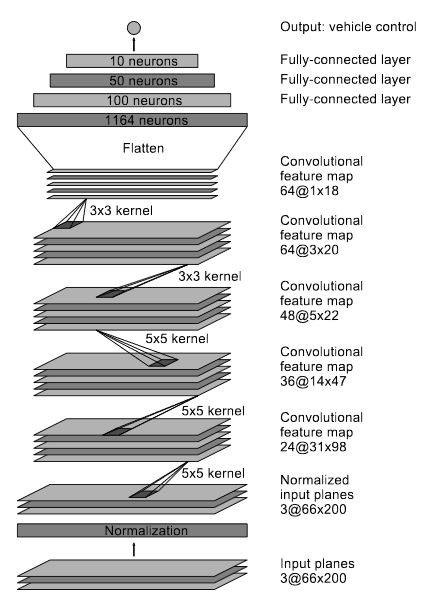
\includegraphics[width=6cm]{nvidiacnn}
	\centering
	\caption{CNN architecture used in \cite{bojarski2016end}. The network contains approximately 27 million connections and 250 thousand parameters.}
	\label{nvidiaimage}
\end{figure}


"Learning Spatiotemporal Features with 3D Convolutional Networks" introduces how to construct 3D Convolutional Networks to capture spatiotemporal features in a sequence of images or videos \cite{Tran_2015_ICCV}. "Beyond Short Snippets: Deep Networks for Video Classification" describes two ways including using LSTM to deal with videos \cite{yue2015beyond}.

"Deep Residual Learning for Image Recognition" \cite{he2016deep} and "Densely Connected Convolutional Networks" \cite{huang2016densely} describe the techniques to construct residual connections between different layers and make it easier to train deep neural networks. 


\section{Methods}

We investigated the top three existing models from the Udacity challenge to study how they work. The first examined model from the challenge is based on Team Komanda's model. The model performs a mapping from sequences of images (or one single video) to sequences of steering angles. Although the target is only the steering angle, this model predicts not only the steering angle, but also the vehicle speed and the torque applied to the steering wheel, which would be used to predict future steering angle. 

The model is consisted by a 3D convolutional stack and a RNN (LSTM) layer after it. The 3D convolutional stack contains four 3D convolutional layers followed by several fully connected layers, converting to a vector with 128 activations in the end. Each 3D convolutional layer will also produce an auxiliary output to be added to the final fully connected layer (residual connect). The output from this 3D convolutional stack will have shape (batch\_size, seq\_len, 128).

How 3D convolutional layer works is similar to 2D conv, the only difference is that in addition to height and width, now we have the third dimension depth. Instead of having a 2D filter (if we ignore the channel dimension for a while) moving within the image along height and width, now we have a 3D filter moving along with height, width and depth. If the input has shape ($D_{1}$, $H_{1}$,  $W_{1}$, $C$), then the output would have shape ($D_{2}$, $H_{2}$, $W_{2}$, $F$) where $F$ is the number of filters. ($D_{2}$, $H_{2}$, $W_{2}$ could be calculated given stride and padding in its dimension.

Combining the output from 3D convolutional layer stack and previous predicted steering angle, torque and speed, we have the input to RNN layer. This input is a tuple of two tensors with shape (batch\_size, seq\_len, 128) and (batch\_size, seq\_len, 3). Based on this input, RNN will make predictions for steering angle, torque and speed. 

The final loss is consisted of major loss from steering angle prediction and auxiliary loss from torque and speed. 
$loss=L2(steering angle)+auxiliary weight*(L2(steering angle)+L2(torque)+L2(speed))$

The L2 loss here is the loss across both batch\_size and seq\_len as we have the true label for each point in the sequence.

During training, we use both ground truth and previous predicted angle, torque and speed as our input to RNN. During testing, we only use previous prediction as the input to RNN.
\begin{figure}[!htb]
	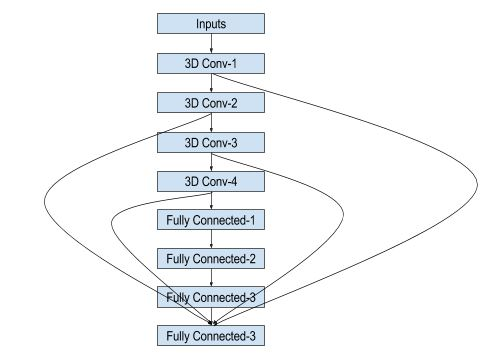
\includegraphics[width=6cm]{Komanda.JPG}
	\centering
	\caption{Architecture used for team Komanda.}
	\label{komanda}
\end{figure}

The next model we examined from the challenge was from Team Rambo. To preprocess the data, the images were converted to grayscale and lag 1 differences between frames were computed. Two consecutive differenced images were used as the input of the model. For example, at time $t, [x_{t} - x_{t-1}, x_{t-1} - x_{t-2}]$ is used as input where x corresponds to the grayscale image. Since two consecutive differenced images were used, the number of channels is 2, but this is a hyperparameter for tuning. 

In the training process, the model consists of 3 streams that are assembled at the final layer. Figure \ref{rambo} shows the architecture of the model. 
\begin{figure}[!htb]
	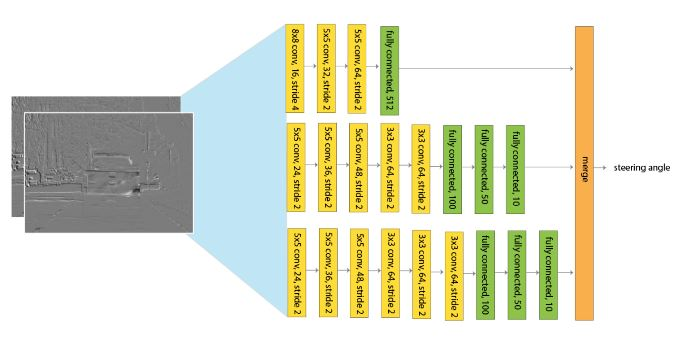
\includegraphics[width=6cm]{rambo.JPG}
	\centering
	\caption{Architecture used for team Rambo.}
	\label{rambo}
\end{figure}
Each stream of the model consists of a sequence of convolutional layers, interspersed with activation functions such as ReLU, Leaky ReLU or Parametric ReLU (PReLU). Adam optimization and L2 loss were adopted as the optimization method and loss equation.

A third model from team Chauffeur was examined. This team placed third with an RMSE of 0.0572. This model had a core structure that was similar to that of team Komanda with the exception of not using 3D convolutional networks. This team used a large pretrained CNN model. This model was then modified to have an output of approximately 3000 features that was then passed into a relatively simple LSTM (long short-term memory \cite{hochreiter1997long}) network with the best model having a window of 50 images or 2.5 seconds of video.

\subsection{3D Convolutional Model}

\subsubsection*{3D Convolutional Layer}
How 3D convolutional layer works is similar to 2D conv, the only difference is that in addition to height and width, now we have the third dimension depth (temporal). Instead of having a 2D filter (if we ignore the channel dimension for a while) moving within the image along height and width, now we have a 3D filter moving along with height, width and depth. If the input has shape (D1, H1,  W1, C), then the output would have shape (D2, H2, W2, F) where F is the number of filters. D2, H2, W2 could be calculated given stride and padding in its dimension.

\subsubsection*{Residual Connection}
Since deep neural network is hard to train, we need residual connections here to help the training process. The idea of residual connection is to use network layers to fit a residual mapping instead of directly trying to fit a desired underlying mapping. 
Without residual connection:
Fit H(G(x)) directly
With residual connection:
Fit $F(x)=H(G(x))-G(x)-x$
After each 3D convolutional layers, we process its output through a fully connected layer and add it to the output of the whole Visual Feature Extraction module.

\subsubsection*{Spatial Batch Normalization}
Batch Normalization alleviates a lot of headaches with properly initializing neural networks by explicitly forcing the activations throughout a network to take on a unit gaussian distribution at the beginning of the training. Spatial batch normalization not only normalize among different samples but also among the spatial axis of images. Here we add spatial batch normalization after each 3D convolutional layer.


\subsection{Transfer Learning}




\subsection{Potential Methods}

A potential method is taking the last $n$ frames from the training set allow use of networks using 3D convolutions \cite{Tran_2015_ICCV}. Creating an architecture like ResNet with these 3D layers may capture important image information between layers and let the gradient pass back deeper into the network. Additionally passing the processed data from this network into an RNN (using LSTM) could allow for knowledge of the previous states to be used to predict the next state of the steering angle. Additional methods that different teams used that could be used with this approach is to take the difference between frames instead of the raw image data. Transfer learning of a large network would also likely be helpful for model development. Ideally, if a high quality simulator can be found, this trained network can modified to be used for deep reinforcement learning. After training in the simulator the model can then be evaluated on the validation and test sets.

\subsection{Data Preprocessing}
During experimentation, copying the general structure from \cite{bojarski2016end} with the dataset from Udacity produced poor results. Initially, training data was passed unprocessed into the model. Without any preprocessing, the RMSE on the training set was very low; however, the error on the validation set was worse than passing all zeros in as the output (0.2130 on the validation set). We are currently examining ways to best augment the training set to improve performance on the validation set. One common idea in the different teams was to flip the training on the $y$ axis to account for any turn asymmetry. Adding random shadows, hue changes, rotations, and shifts in the images are being examined along with incorporation images from the left and right cameras. However, using the left and right cameras when using RNNs may not make sense as the angle is interpolated as what the car should do if that image were the front facing camera. Frames that have the steering angle at approximately 0 can be preferentially excluding in favor of frames with larger steering angles.


\section{Dataset and Features}
The dataset we used is provided by Udacity, which is generated by NVIDIA’s DAVE-2 System \cite{bojarski2016end}. Specifically, three cameras are mounted behind the windshield of the data-acquisition car. Time-stamped video from the cameras is captured simultaneously with the steering angle applied by the human driver. This steering command is obtained by tapping into the vehicle’s Controller Area Network (CAN) bus. In order to make the system independent of the car geometry, they represent the steering command as 1/r where r is the turning radius in meters. They use 1/r instead of r to prevent a singularity when driving straight (the turning radius for driving straight is infinity). 1/r smoothly transitions through zero from left turns (negative values) to right turns (positive values). Training data contains single images sampled from the video, paired with the corresponding steering command (1/r).

In addition to the images got from the center camera, images for two specific off-center shifts can be obtained from the left and the right camera. Additional shifts between the cameras and all rotations are simulated by viewpoint transformation of the image from the nearest camera. This could be regarded as a way we used to augment the data.

Raw images are of size 640 x 480 and have three channels RGB. For one of our models, we resized the images to 256 x 192, converted from RGB color format to grayscale, computed lag 1 differences between frames and used 2 consecutive differenced images. For example, at time t we used $[x_{t} - x_{t-1}, x_{t-1} - x_{t-2}]$ as input where x corresponds to the grayscale image.

Training data set contains 101397 frames and corresponding labels including steering angle, torque and speed. We further split this data set into training and validation in a 80/20 fashion. And there is also a test set which contains 5615 frames. 

\section{Experiments, Results, and Discussion}

\subsection{Data Augmentation}
In order to establish a baseline for our research, we used the architecture from \cite{bojarski2016end} to test different forms of data augmentation. Teams in the Udacity challenge noted that data augmentation was helpful along with the original NVIDIA researchers. Knowing which forms of augmentation work well for the amount of time and computational available would be helpful in training our new models.

Three different levels of augmentation were examined. The first had minimal augmentation with only using random flips and cropping of the top of the image. Randomly flipping the input images eliminates the bias towards right turns found in the dataset. Cropping the top of the image eliminates the sky from the image, which should not play a role in how to turn predict the steering angle. A second form of augmentation had the same augmentation as the minimal version along with small rotations (-5 to +5 degrees), shifts (25 pixels), and small brightness changes of the image. The final Heavier version of augmentation used more exaggerated effects of the second version including large angle rotations (up to 30 degrees), large shadows, shifts, and larger brightness changes were used. Results from this experiment can be see in Table \ref{data_aug_table}.

\begin{table}[!htb]
	\centering
	\caption{RMSE on the validation set using the NVIDIA architecture for different levels of data augmentation with 32 epochs.}
	\label{data_aug_table}
	\begin{tabular}{|l|l|l|}
		\hline
		\textbf{Minimal} & \textbf{Moderate} & \textbf{Heavy} \\ \hline
		0.09             & 0.10              & 0.19           \\ \hline
	\end{tabular}
\end{table}
 
Using heavy data augmentation produced very poor results that were not much above predicting a steering angle of 0 for all the data. The moderate augmentation produced good results; however the minimal augmentation produced the best results. These results could be explained by only training for 32 epochs. Heavy augmentation could be hard for the model to pick up on such drastic shifts. Similarly, the moderate version could have outperformed the minimal version over more epochs. What these models find important can be visualized through saliency maps (see Figure \ref{nvidia_aug}). 
 
 \begin{figure}[!htb]
 	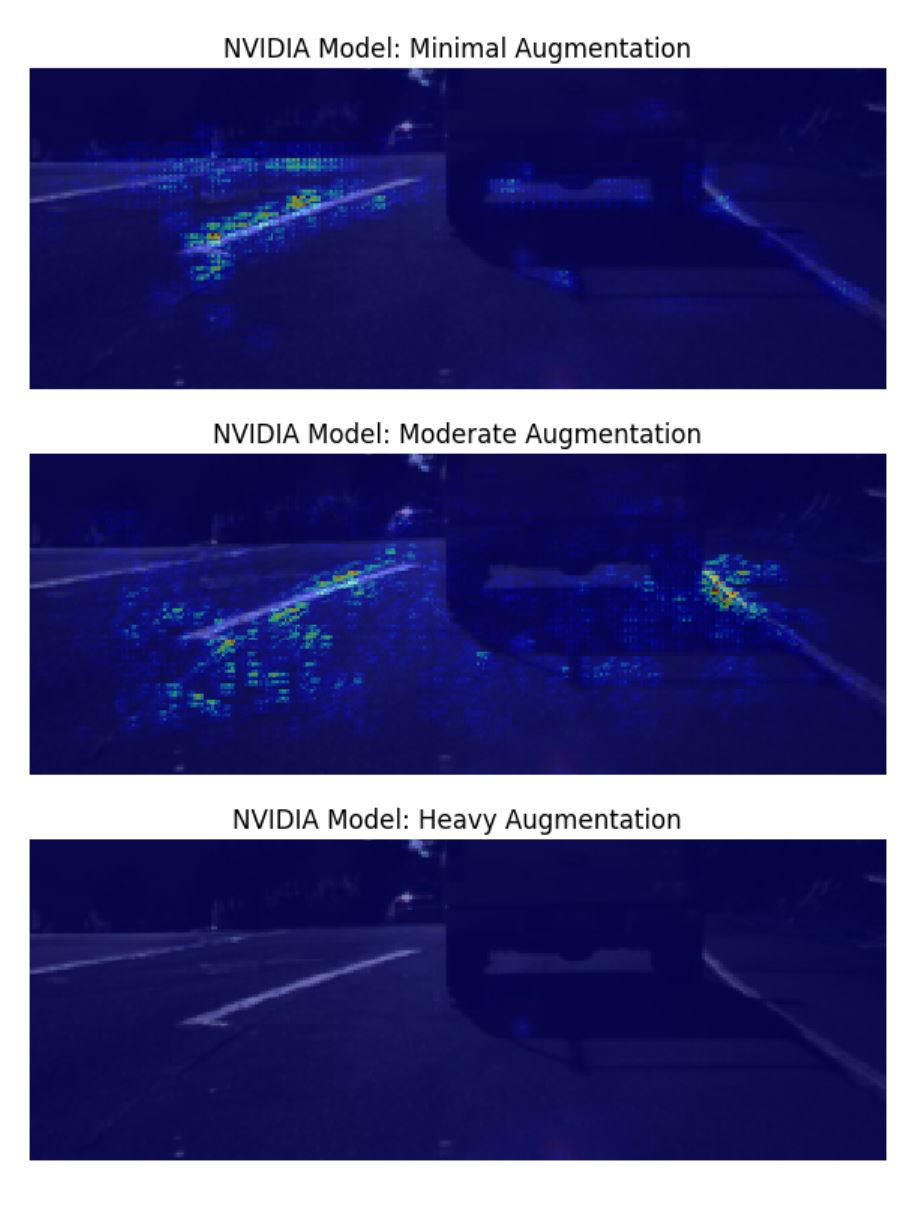
\includegraphics[width=8cm]{nvidia_aug_test_vert.png}
 	\centering
 	\caption{NVIDIA model saliency maps for different levels of augmentation.}
 	\label{nvidia_aug}
 \end{figure}
 
The minimal model found the lanes important. In the moderate model more of the lane markers were found to be important, but this model's saliency maps appeared more noisy, which could explain its slightly decreased performance. In the heavy model almost no areas were found to be salient, which is understandable due to its poor performance. For our new models, we chose to use minimal augmentation.


\subsection{Transfer Learning}
For this model, we used transfer learning. Of the pre-trained models available, ResNet50 had good performance for this dataset. This model was trained on ImageNet. The weights of the first 15 ResNet blocks were blocked from updating (first 45 individual layers out of 175 total). The output of ResNet50 was connected to a stack of fully connected layers containing 512, 256, 64, and 1 different units respectively. The architecture of this model can be seen in Figure \ref{resnet50}. Other sizes were attempted, but produced either poor results or were slow in training. For example, training only the last 5 blocks provided poor results, which were only slightly better than predicting a steering angle of zero for all inputs. The model took as input images of 224x224x3. The only augmentation provided for this model was mirrored images. Due to the size constraints of the input into ResNet50, cropping involved stretching the image. The filters in the pretrained model were not trained on stretched images, so the filters may not activate as well on the stretched data (RMSE of 0.0891 on the validation set after 32 epochs). Additionally, using the left and the right cameras from the training set proved not to be useful for the 32 epochs used to train (0.17 RMSE on the validation set).

\begin{figure}[!htb!]
	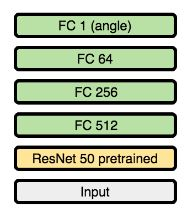
\includegraphics[width=4cm]{resnet50trans.JPG}
	\centering
	\caption{Architecture used for transfer learning model.}
	\label{resnet50}
\end{figure}

 \begin{figure}[!htb]
	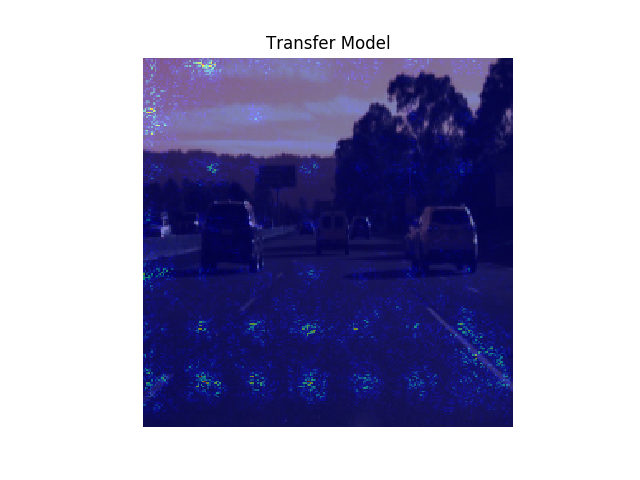
\includegraphics[width=8cm]{resnet50trans_saliency.png}
	\centering
	\caption{Transfer learning model (ResNet50) saliency map for an example image.}
	\label{resnet50_saliency}
\end{figure}

An example saliency map for this model can be seen in Figure \ref{resnet50_saliency}. The model does appear to have salient features on the road markers; however, there are also regularly spaced blotches. These blotches may be artifacts from using this type pretrained model with residual connections. The results of the transfer learning model had a RMSE on the validation set of 0.0775 and a test set RMSE of 0.0709. For reference, this model would have placed fourth in the Udacity challenge. Overall, this strategy of using a pre-trained model, locking approximately the first quarter layers, training the deeper layers with the existing weights, and connecting to a fully connected stack proved to be effective in producing a high quality and competitive model for the Udacity self-driving car dataset.


\subsection{New 3D Architecture}
For self driving cars, incorporating temporal information could play an important role in production systems. For example, if the camera sensor is fully saturated looking at the sun, knowing the information of the previous frames would allow for a much better prediction than basing the steering angle prediction only on the saturated frame. As discussed earlier, 3D convolutional layers and recurrent layers incorporate temporal information. In this model we combined these two ways of using temporal information. We used the idea residual connection in constructing this model \cite{he2016deep}. These connections allow for more of the gradient to pass through network by combining different layers. The model consisted five sequences of five frames of video shifted by one frame for the input (5x5x120x320x3). The values were selected to fit the computational budget. This allowed for both motion and differences in outputs between frames to be used. The architecture of the model can be seen in Figure \ref{3dconvlstm_graph}.

 \begin{figure}[!htb]
	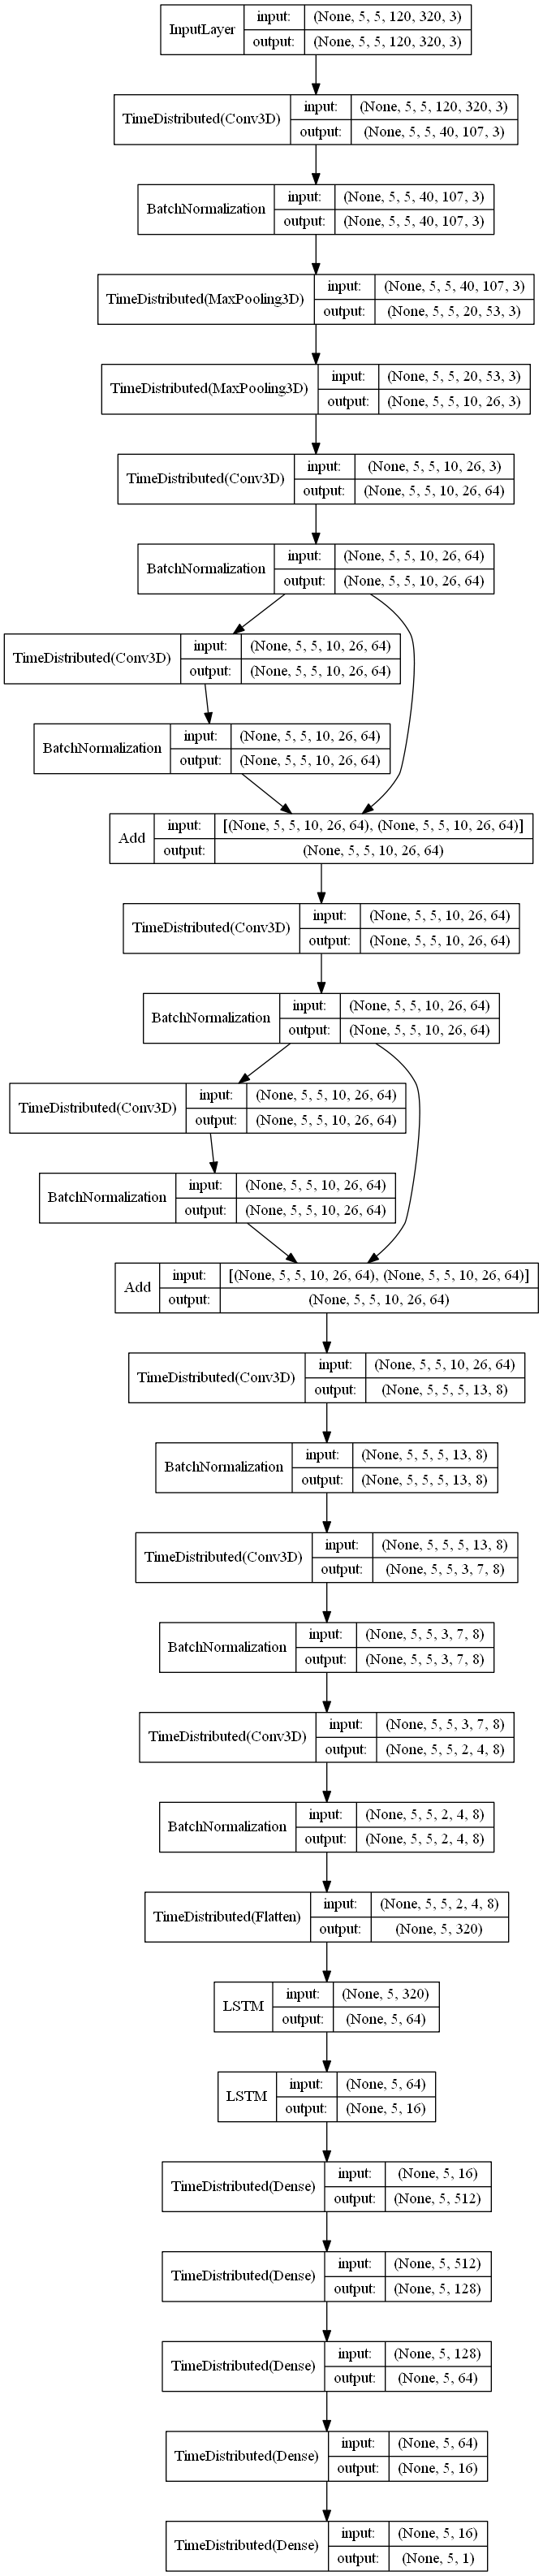
\includegraphics[width=2cm]{3dlstmv2.png}
	\centering
	\caption{3D convolutional model with residual connections and recurrent LSTM layers}
	\label{3dconvlstm_graph}
\end{figure}

The model consists of a few initial layers to shrink the size followed by ResNet like blocks of 3D convolutions with spatial batch normalization (only two of these in the trained model). Due to computational restraints, shrink layers were added to make the input to the fully connected layers much smaller. Even with the computational restraints, this RMSE for this model on the test set was 0.1123 (trained for 32 epochs), which would have placed tenth in the Udacity challenge.

%\begin{figure}[!htb]
%	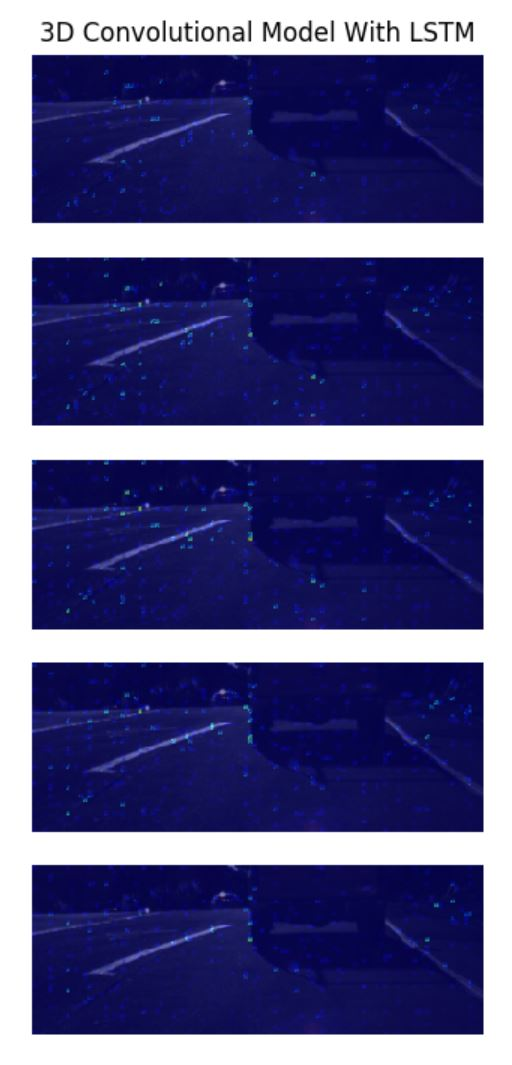
\includegraphics[width=6cm]{3d_lstm_full_title.png}
%	\centering
%	\caption{Transfer learning model (ResNet50) saliency map for example image.}
%	\label{3d_full}
%\end{figure}

\begin{figure}[!htb]
	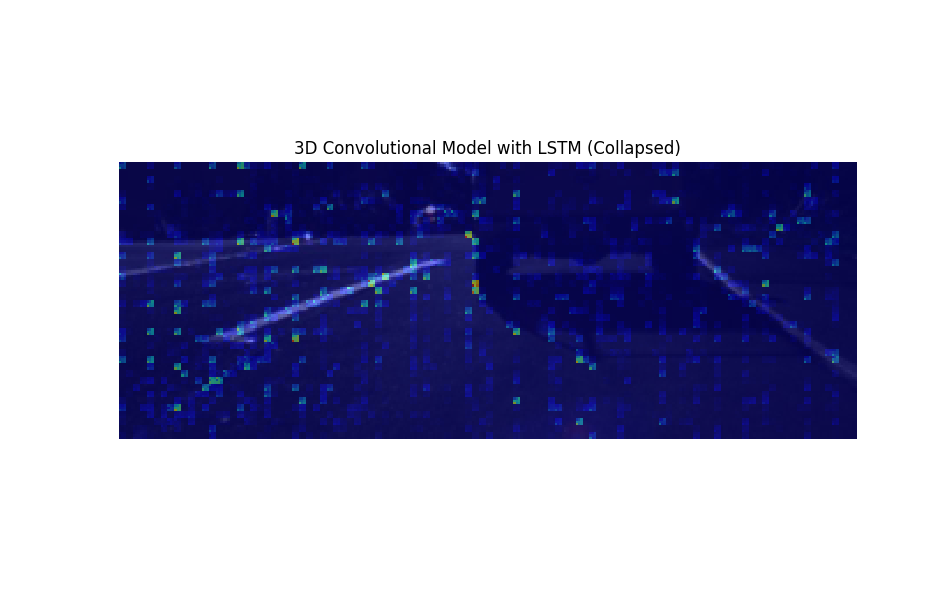
\includegraphics[width=8cm]{3d_full_v2_collapsed.png}
	\centering
	\caption{Saliency map for the 3D convolutional model with residual connections and recurrent LSTM layers for an example image.}
	\label{3d_collapse}
\end{figure}

This model produced interesting saliency maps. The collapsed version of the maps, where all the frames are merged into a single image, is shown in Figure \ref{3d_collapse}. The salient features seem to be changes from frame to frame. These do cluster around road markers, but they also cluster around other vehicles and their shadows. This model may be using information about the card in front in order to make a steering angle prediction along with the road markers. Overall, this new method showed that it could have competitive results. With more time and computational resources, this model could have been expanded to take in a longer period of video along with more ResNet blocks. Expanding the model in this way could have produced superior results.




\subsection{Results}



\section{Conclusion and Future Work}

In examining the final leader board from Udacity our models would have placed fourth (transfer learning model) and tenth (3D convolutional model with LSTM layers). These results were produced solely from the models without any external smoothing function. We have shown that both transfer learning and a more advanced architecture have promise in the field of autonomous vehicles. The 3D model was limited by computational resources, but overall still provided a good result from a novel architecture. In future work the 3D model's architecture could be expanded by having a larger and deeper layers, which may produce better results.

These models are far from perfect and there is substantial research that still needs to be done on the subject before models like these can be deployed widely to transport the public. These models may benefit from a wider range of training data. For a production system, a model would have to be able to handle the environment in snowy conditions. Generate adversarial models, GANs, could be used to transform a summer training set into a winter one. Additionally, GANs could be used to generate more scenes with sharp angles. Additionally, a high quality simulator could be used with deep reinforcement learning. A potential reward function could be getting from one point to another while minimizing time, maximizing smoothness of the ride, staying in the correct lane/following the rules of the road, and not hitting objects.




{\small
\bibliographystyle{ieee}
\bibliography{egbib}
}

\end{document}
